\documentclass{article}
\usepackage{expl3}
\usepackage{xparse}
\usepackage[dvipsnames]{xcolor}
\usepackage{pgfplots}
\usepackage[T1]{fontenc}
\usepackage{frcursive}
\usepackage{calligra}

% Required to support mathematical unicode
\usepackage[warnunknown, fasterrors, mathletters]{ucs}
\usepackage[english]{babel}
% Always typeset math in display style
\everymath{\displaystyle}

% Standard mathematical typesetting packages
\usepackage{amsfonts, amsthm, amsmath, amssymb}
\DeclareMathSymbol{\shortminus}{\mathbin}{AMSa}{"39}
\usepackage{mathtools}  % Extension to amsmath
\usepackage[fontsize=14pt]{scrextend}

% Symbol and utility packages
\usepackage{cancel, textcomp}
\usepackage[mathscr]{euscript}
\usepackage[nointegrals]{wasysym}

% Extras
\usepackage{physics}  % Lots of useful shortcuts and macros
\usepackage{tikz-cd}  % For drawing commutative diagrams easily
\usetikzlibrary{angles}
\usepackage{color}  % Add some colour to life
\usepackage{microtype}  % Minature font tweaks
\usepackage{mathrsfs}  % For curly sets
\usepackage{polynom}


\usepackage{soul}
\usepackage[version=4]{mhchem}
\usepackage{esint}
\usepackage{tikz-3dplot}

\usepackage{tikz-feynman}
\usepackage[colorlinks]{hyperref}
\usepackage{enumerate}
\usepackage{tcolorbox}
\usepackage{enumitem}

\begin{document}

\subsection*{Quotient Identity} $$\tan \theta=\frac{\sin \theta}{\cos \theta}$$

\subsection*{Geometry Trigonometry Definition}
 \def\angle{52}

  \pgfmathsetmacro{\r}{1}
  \pgfmathsetmacro{\s}{sin(\angle)}
  \pgfmathsetmacro{\c}{cos(\angle)}
  %colors
  \definecolor{r}{HTML}{ff3030}
  \definecolor{b}{HTML}{00bfff}
  \definecolor{o}{HTML}{ff7e00}
  \definecolor{g}{HTML}{50C878}

  \begin{tikzpicture}[scale=5,very thick]

    % grey axis
    \draw[gray!30] (0, 0) -- (0, 1/\s+.1);
    \draw[gray!30] (0, 0) -- (1/\c+.1, 0);

    % arc of the angle
    \draw (1/5,0) node[sloped,anchor=south east] {$\theta$} arc (0:\angle:1/5);

    % radius 1, cos and sin
    \draw (0, 0) --node [sloped, above]{1} (\angle:1);
    \draw (0, \s) -- node [below]{$\cos(\theta)$} (\c,\s);
    \draw (\c, \s)-- node [right]{$\sin(\theta)$}(\c,0);

    % quarter circle:
    \draw (1,0) arc(0:90:1);

    % big triangle: sec(x), tan(x), csc(x), cot(x)
    \draw [r] (0, 0) -- node [below] {$\sec(\theta)$} (1/\c,0);
    \draw [b] (1/\c, 0) -- node [sloped,above] {$\tan(\theta)$} (\c,\s);
    \draw [o] (0, 0) -- node [left=1mm] {$\csc(\theta)$} (0,1/\s);
    \draw [g] (0, 1/\s) -- node [sloped,above] {$\cot(\theta)$} (\c,\s);
  \end{tikzpicture}

\subsection*{Double angle}
  \begin{align*}
    \cos (2\theta) &= \cos^2(\theta) - \sin^2(\theta) \\
      &= 2\cos^2(\theta) - 1 \\
      &= 1 - 2\sin^2(\theta) \\
    \sin(2\theta) &= 2\sin(\theta)\cos(\theta) \\
    \tan(2\theta) &= \frac{2\tan(\theta)}{1-\tan^2(\theta)}
  \end{align*}
  
\subsection*{Half-Angle}
  \begin{align*}
    \sin(\tfrac{\theta}{2}) &= \pm\sqrt{\tfrac{1-\cos(\theta)}{2}} \\
    \cos(\tfrac{\theta}{2}) &= \pm\sqrt{\tfrac{1+\cos(\theta)}{2}} \\
    \tan(\tfrac{\theta}{2}) &= \pm\sqrt{\tfrac{1-\cos(\theta)}{1+\cos(\theta)}}
  \end{align*}
\subsection*{Sum and Difference}
\begin{align*}
\sin (\theta \pm \varphi) &= \sin(\theta)\cos(\varphi) \pm \cos(\theta)\sin(\varphi) \\
\cos (\theta \pm \varphi) &= \cos(\theta)\cos(\varphi) \mp \sin(\theta)\sin(\varphi) \\
\tan (\theta \pm \varphi) &= \frac{\tan(\theta) \pm \tan(\varphi)}{1 \mp \tan(\theta)\tan(\varphi)}
\end{align*}

\subsection*{Pythagorean Identity} $\sin ^2 \theta+\cos ^2 \theta=1$ (from the unit circle)

\subsection*{Reciprocal Identities }
$$
\begin{array}{ll}
\csc \theta=\frac{1}{\sin \theta} ; \quad \sin \theta=\frac{1}{\csc \theta} \\\\
\sec \theta=\frac{1}{\cos \theta} ; \quad \cos \theta=\frac{1}{\sec \theta} \\\\
\tan \theta=\frac{1}{\cot \theta} ; \quad \cot \theta=\frac{1}{\tan \theta}
\end{array}
$$

\subsection*{Compound Angle Formulas:}
$$
\begin{aligned}
\sin (\alpha+\beta) & =\sin \alpha \cos \beta+\cos \alpha \sin \beta \\
\sin (\alpha-\beta) & =\sin \alpha \cos \beta-\cos \alpha \sin \beta \\
\cos (\alpha+\beta) & =\cos \alpha \cos \beta-\sin \alpha \sin \beta \\
\cos (\alpha-\beta) & =\cos \alpha \cos \beta+\sin \alpha \sin \beta\\
\tan (\alpha+\beta)&=\frac{\tan \alpha+tan \beta}{1-\tan \alpha\tan\beta}\\
\tan (\alpha-\beta)&=\frac{\tan \alpha-tan \beta}{1+\tan \alpha\tan\beta}
\end{aligned}
$$
\subsection*{Reciprocal of Trigonometry}
  \begin{spreadlines}{1.5ex}
    \begin{alignat*}{2}
      \csc(x) & = \tfrac 1 {\sin(x)}, \quad & \tan(x) & = \tfrac {\sin(x)} {\cos(x)} \\
      \sec(x) & = \tfrac 1 {\cos(x)}, \quad & \cot(x) & = \tfrac {\cos(x)} {\sin(x)}
    \end{alignat*}
  \end{spreadlines}
\subsection*{Reflection in trigonometry}
  \begin{spreadlines}{1.5ex}
    \begin{alignat*}{3}
      \sin(-x) &= -\sin(x), \quad & \sin(\tfrac\pi2 - x) &= \cos(x), \quad & \sin(\pi - x) &= \hphantom-\sin(x) \\
      \cos(-x) &= \hphantom-\cos(x), \quad & \cos(\tfrac\pi2 - x) &= \sin(x), \quad & \cos(\pi - x) &= -\cos(x) \\
      \tan(-x) &= -\tan(x), \quad & \tan(\tfrac\pi2 - x) &= \tfrac1{\tan(x)}, \quad & \tan(\pi - x) &= -\tan(x)
    \end{alignat*}
  \end{spreadlines}
\subsection*{Shift in Trigonometry}
  \begin{spreadlines}{1.5ex}
    \begin{alignat*}{2}
      \sin\left(\frac\pi2 + x\right) &=  \cos(x), \quad & \sin\left(\pi + x\right) &= -\sin(x) \\
      \cos\left(\frac\pi2 + x\right) &= -\sin(x), \quad & \cos\left(\pi + x\right) &= -\cos(x) \\
      \tan\left(\frac\pi2 + x\right) &= -\frac{1}{\tan(x)}, \quad & \tan\left(\pi + x\right) &=  \tan(x)
    \end{alignat*}
  \end{spreadlines}

\subsection*{Reflection of Shift Trigonometry}
  \setbox2=\hbox{\vrule height3.5ex depth3ex width0pt}
  \halign{
    \unhcopy2\strut#&\vrule#\tabskip=1em&\hfil$#$\hfil&\vrule#&\hfil$#$\hfil&\vrule#&\hfil$#$\hfil&\vrule#&\hfil$#$\hfil&\vrule#&\hfil$#$\hfil&#\vrule\tabskip=0pt\cr
    \noalign{\hrule}
    &&\theta&&\frac{\pi}{2} - x&&\frac{\pi}{2} + x&&\pi - x&&\pi +x&\cr
    \noalign{\hrule}
    &&\sin(\theta)&&\cos(x)&&\cos(x)&&\sin(x)&&-\sin(x)&\cr
    \noalign{\hrule}
    &&\cos(\theta)&&\sin(x)&&-\sin(x)&&-\cos(x)&&-\cos(x)&\cr
    \noalign{\hrule}
    &&\tan(\theta)&&\frac{1}{\tan(x)}&&\frac{-1}{\tan(x)}&&-\tan(x)&&\tan(x)&\cr
    \noalign{\hrule}
  }
\vspace{1em}
  
\subsection*{Sum-to-Product Formulas}
  \begin{spreadlines}{1.3ex}
    \begin{alignat*}{3}
      &\cos(x) + \cos(y)\ &=\ &\, 2\cos(\tfrac{x + y}2)\cos(\tfrac{x - y}2) \\
      &\cos(x) - \cos(y)\ &=\ &\, 2\sin(\tfrac{x + y}2)\sin(\tfrac{y - x}2) \\
      &\sin(x) + \sin(y)\ &=\ &\, 2\sin(\tfrac{x + y}2)\cos(\tfrac{x - y}2) \\
      &\sin(x) - \sin(y)\ &=\ &\, 2\cos(\tfrac{x + y}2)\sin(\tfrac{x - y}2) \\
    \end{alignat*}
  \end{spreadlines}  
  \subsection*{Product-to-sum formulas}
    \begin{spreadlines}{1ex}
    \begin{alignat*}{3}
      &2\sin(x)\sin(y)\ &=\ & \cos(x-y)-\cos(x + y) \\
      &2\sin(x)\cos(y)\ &=\ & \sin(x + y) + \sin(x - y) \\
      &2\cos(x)\cos(y)\ &=\ & \cos(x + y) + \cos(x - y)
    \end{alignat*}
  \end{spreadlines}
\subsection*{Related Angle Identities}

\begin{align*}
&\sin (\pi - \theta) = \sin \theta \quad
&&\sin (\pi + \theta) = -\sin \theta \\
&\sin (2\pi - \theta) = -\sin \theta \quad
&&\sin (-\theta) = -\sin \theta \\
&\cos (\pi - \theta) = -\cos \theta \quad
&&\cos (\pi + \theta) = -\cos \theta \\
&\cos (2\pi - \theta) = \cos \theta \quad
&&\cos (-\theta) = \cos \theta \\
&\tan (\pi - \theta) = -\tan \theta \quad
&&\tan (\pi + \theta) = \tan \theta \\
&\tan (2\pi - \theta) = -\tan \theta \quad
&&\tan (-\theta) = -\tan \theta
\end{align*}


\subsection*{Co-related Angle Identities}
\begin{align*}
&\sin \left(\frac{\pi}{2} - \theta\right) = \cos \theta \quad
&&\sin \left(\frac{\pi}{2} + \theta\right) = \cos \theta \\
&\sin \left(\frac{3\pi}{2} - \theta\right) = -\cos \theta \quad
&&\sin \left(\frac{3\pi}{2} + \theta\right) = -\cos \theta \\
&\cos \left(\frac{\pi}{2} - \theta\right) = \sin \theta \quad
&&\cos \left(\frac{\pi}{2} + \theta\right) = -\sin \theta \\
&\cos \left(\frac{3\pi}{2} - \theta\right) = -\sin \theta \quad
&&\cos \left(\frac{3\pi}{2} + \theta\right) = \sin \theta \\
&\tan \left(\frac{\pi}{2} - \theta\right) = \cot \theta \quad
&&\tan \left(\frac{\pi}{2} + \theta\right) = -\cot \theta \\
&\tan \left(\frac{3\pi}{2} - \theta\right) = \cot \theta \quad
&&\tan \left(\frac{3\pi}{2} + \theta\right) = -\cot \theta
\end{align*}


\newpage 
 \subsection*{Long list of trig identities}
  \textbf{Defining relations:} \hspace{3cm} $\approx \mathcal{O}\omega \mathcal{O}\approx$
  \begin{flalign*}
    &\quad \csc(x) = \tfrac1{\sin(x)}\quad\tan(x) = \tfrac{\sin(x)}{\cos(x)} &\\
    &\quad \sec(x) = \tfrac1{\cos(x)}\quad\cot(x) = \tfrac1{\tan(x)} = \tfrac{\cos(x)}{\sin(x)}&
  \end{flalign*}
  \textbf{Pythagoras:}
  \begin{flalign*}
    &\quad \sin^2(x) + \cos^2(x) = 1 &\\
    &\quad 1 + \cot^2(x) = \csc^2(x) &\\
    &\quad \tan^2(x) + 1 = \sec^2(x)&
  \end{flalign*}
  \textbf{Cofunction, Negative angle, and Supplement:}
  \begin{flalign*}
    &\quad \sin(x) = \cos(\tfrac\pi2-x)\quad\sin(-x) = -\sin(x) &\\
    &\quad \cos(x) = \sin(\tfrac\pi2-x)\quad\cos(-x) = \cos(x) &\\
    &\quad \tan(x) = \cot(\tfrac\pi2-x)\quad\tan(-x) = -\tan(x) &\\
    &\quad \sin(\pi-x) = \sin(x) &\\
    &\quad \cos(\pi-x) = -\cos(x) &\\
    &\quad \tan(\pi-x) = -\tan(x) &
  \end{flalign*}
  \textbf{Periodicity: for all $n\in\mathbb{Z}$} 
  \begin{flalign*}
    &\quad \sin(x + 2\pi n) = \sin(x) &\\
    &\quad \cos(x + 2\pi n) = \cos(x) &\\
    &\quad \tan(x + \pi n) = \tan(x) &
  \end{flalign*}
  \textbf{Addition:}
  \begin{flalign*}
    &\quad \sin(x\pm y) = \sin(x)\cos(y)\pm\cos(x)\sin(y) &\\
    &\quad \cos(x\pm y) = \cos(x)\cos(y)\mp\sin(x)\sin(y) &\\
    &\quad \tan(x\pm y) = \tfrac{\tan(x)\pm\tan(y)}{1\mp\tan(x)\tan(y)} &
  \end{flalign*}
  \textbf{Double angle:}
  \begin{flalign*}
    &\quad \sin(2x) = 2\sin(x)\cos(x) &\\
    &\quad \cos(2x) = \cos^2(x)-\sin^2(x) \\
    &\quad \cos(2x) = 2\cos^2(x)-1 = 1-2\sin^2(x) &\\
    &\quad \tan(2x) = \tfrac{2\tan(x)}{1-\tan^2(x)} &
  \end{flalign*}
  \textbf{Sum--to--product and Product--to--sum:}
  \begin{flalign*}
    &\quad \cos(x) + \cos(y) = 2\cos(\tfrac{x + y}2)\cos(\tfrac{x-y}2) &\\
    &\quad \cos(x)-\cos(y) = -2\sin(\tfrac{x + y}2)\sin(\tfrac{x-y}2) &\\
    &\quad \sin(x)\pm\sin(y) = 2\sin(\tfrac{x\pm y}2)\cos(\tfrac{x\mp y}2) &\\
    &\quad 2\sin(x)\sin(y) = \cos(x-y)-\cos(x + y) &\\
    &\quad 2\sin(x)\cos(y) = \sin(x + y) + \sin(x - y) &\\
    &\quad 2\cos(x)\cos(y) = \cos(x + y) + \cos(x - y) &
  \end{flalign*}

\subsection*{Special Triangles and the Unit Circle}
\begin{figure}[ht]
    \centering
    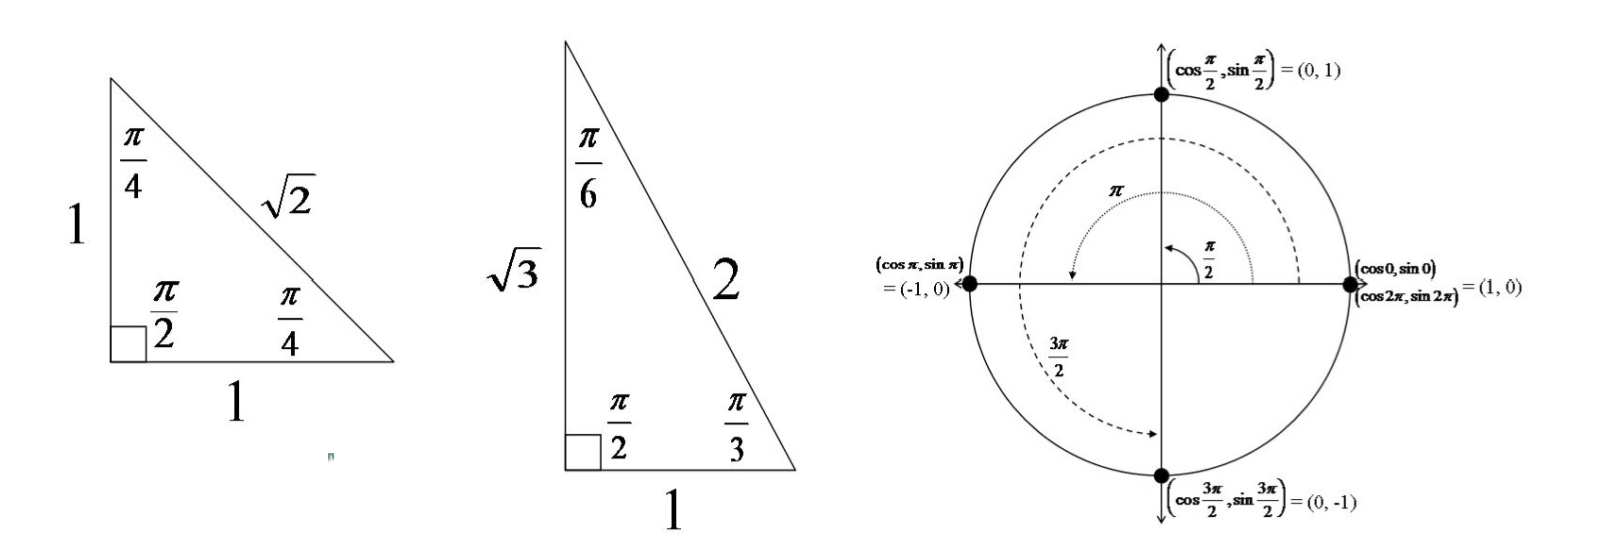
\includegraphics[width=1\textwidth]{imgs/special trig and the unit circle.png}
\end{figure}
  
\subsection*{Unit Circle}  
  \begin{tikzpicture}[scale=4.5, font=\small]
  \definecolor{r}{HTML}{ff3030}
  \definecolor{b}{HTML}{00bfff}
  \definecolor{o}{HTML}{DA70D6}
  \def\angles{
      0/2\pi/1/0/0,
      30/\frac{\pi}{6}/\frac{\sqrt{3}}{2}/\frac{1}{2}/\frac{\sqrt{3}}{3},
      45/\frac{\pi}{4}/\frac{\sqrt{2}}{2}/\frac{\sqrt{2}}{2}/1,
      60/\frac{\pi}{3}/\frac{1}{2}/\frac{\sqrt{3}}{2}/\sqrt{3},
      90/\frac{\pi}{2}/0/1/\text{Undefined},
      120/\frac{2\pi}{3}/-\frac{1}{2}/\frac{\sqrt{3}}{2}/-\sqrt{3},
      135/\frac{3\pi}{4}/-\frac{\sqrt{2}}{2}/\frac{\sqrt{2}}{2}/-1,
      150/\frac{5\pi}{6}/-\frac{\sqrt{3}}{2}/\frac{1}{2}/-\frac{\sqrt{3}}{3},
      180/\pi/-1/0/\text{-1},
      210/\frac{7\pi}{6}/-\frac{\sqrt{3}}{2}/-\frac{1}{2}/\frac{\sqrt{3}}{3},
      225/\frac{5\pi}{4}/-\frac{\sqrt{2}}{2}/-\frac{\sqrt{2}}{2}/1,
      240/\frac{4\pi}{3}/-\frac{1}{2}/-\frac{\sqrt{3}}{2}/\sqrt{3},
      270/\frac{3\pi}{2}/0/-1/\text{Undefined},
      300/\frac{5\pi}{3}/\frac{1}{2}/-\frac{\sqrt{3}}{2}/-\sqrt{3},
      315/\frac{7\pi}{4}/\frac{\sqrt{2}}{2}/-\frac{\sqrt{2}}{2}/-1,
      330/\frac{11\pi}{6}/\frac{\sqrt{3}}{2}/-\frac{1}{2}/-\frac{\sqrt{3}}{3}
  }
  \begin{scope}[every node/.style={inner sep=1pt, outer sep=0pt}]
      \foreach \a/\at/\x/\y/\t in \angles {
          \begin{pgfinterruptboundingbox}
              \node (x) at (\a : 1.15) [anchor=\a-180] {\phantom{$\textstyle\left({\color{b} \x}, {\color{o} \y}, {\color{r} \t}\right)$}};
              \clip [rounded corners] (x.south west) rectangle (x.north east) (-1.6, -1.6) -- (1.6, -1.6) -- (1.6, 1.6) -- (-1.6, 1.6) -- cycle;
              \node (x) at (\a : 0.85) [anchor=\a] {\phantom{$\textstyle\at$}};
              \clip [rounded corners] (x.south west) rectangle (x.north east) (-1.6, -1.6) -- (1.6, -1.6) -- (1.6, 1.6) -- (-1.6, 1.6) -- cycle;
              \node (x) at (\a : 0.65) [anchor=\a, font=\footnotesize] {\phantom{$\textstyle\a^\circ$}};
              \clip [rounded corners] (x.south west) rectangle (x.north east) (-1.6, -1.6) -- (1.6, -1.6) -- (1.6, 1.6) -- (-1.6, 1.6) -- cycle;
              \clip (\a : 1) circle [radius=.5pt] (-1.6, -1.6) -- (-1.6, 1.6) -- (1.6, 1.6) -- (1.6, -1.6) -- cycle;
          \end{pgfinterruptboundingbox}
      }

      \draw [r, thick] (-1.5, 0) edge [-{Classical TikZ Rightarrow[length=5pt, width=6pt]}] (1.5, 0) node at (1.5, 0) [right=5pt] {$\textstyle\color{b} x$}
      (0, -1.5) edge [-{Classical TikZ Rightarrow[length=5pt, width=6pt]}] (0, 1.5) node at (0, 1.5) [above=5pt] {$\textstyle\color{o} y$};
      \draw [very thick] (0, 0) circle [radius=1];

      \foreach \a/\at/\x/\y/\t in \angles { \draw [opacity=.4] (0, 0) -- (\a : 1); }
  \end{scope}

  \scoped [every node/.style={inner sep=1pt, outer sep=0pt}] {
      \foreach \a/\at/\x/\y/\t in \angles {
          \node at (\a : 1.15) [anchor=\a-180, rounded corners] {$\textstyle\left({\color{b} \x}, {\color{o} \y}, {\color{r} \t}\right)$};
          \node at (\a : 0.85) [anchor=\a, rounded corners] {$\textstyle\at$};
          \node at (\a : 0.65) [anchor=\a, rounded corners, font=\footnotesize] {$\textstyle\a^\circ$};
          \draw [thick] (\a : 1) circle [radius=.5pt];
      }
  }

  \node at (1, 1.5) [thick, draw=r, rounded corners=6pt] {$\textstyle\left({\color{b} \cos(\theta)}, {\color{o} \sin(\theta)}, {\color{r} \tan(\theta)}\right)$};
    % \node at (0, 1.8) [font={\Huge\sffamily}] {Unit Circle};
  \end{tikzpicture}
\end{document}
